\exercise{Control}
In robotic locomotion it is common to abstract from the robot by using inverted pendulum models.
In this exercise we will use a planar double inverted pendulum to test different control strategies. Our robot can be controlled by specifying the torque $\mathbf{u}=[u_1, u_2]$ of its motors. Consider that in mechanical systems the torque $\vec{u}$ is a function of the joint positions $\vec{q}$, velocities $\dot{\vec{q}}$ and accelerations $\ddot{\vec{q}}$, as given by  
\[
\vec{u}=\vec{M}(\vec{q})\ddot{\vec{q}}+\vec{c}(\vec{q},\dot{\vec{q}})+\vec{g}(\vec{q}), 
\] 
where $\vec{M}$ denotes the inertial matrix, $\vec{c}(\vec{q},\dot{\vec{q}})$ the Coriolis and centripetal forces, and $\vec{g}$ the gravity terms. In the following exercises assume that these terms are given.

For the programming exercises you will use the attached code. 
We provide skeletons for controlling the system either in joint space (\texttt{my\_ctl.py}) or in task space (\texttt{my\_taskSpace\_ctl.py}) and a basic functionality for plotting. You can invoke either mode by running \texttt{jointCtlComp.py} or \texttt{taskCtlComp.py} respectively. 
Attach a printout with plots and a snippet of your source code for each programming exercise. 

\begin{questions}
	
	%----------------------------------------------
	
	\begin{question}{PID Controller}{2}
		What is the form of a proportional-integral-derivative (PID) controller and how could you use it to control a robot, i.e. what physical quantities could you control? Name one positive and one negative aspect of PID controllers.
		
\begin{answer}
A PID controller comes in the form of: \begin{align*}
	u=K_{\textrm{p}} (q_{\textrm{des}} - q) + K_{\textrm{D}} (\dot{q_{\textrm{des}}} - \dot{\textrm{q}}) + K_{\textrm{I}} \int_{-\infty}^{t}(q_{\textrm{des}} - q)\textrm{d}\tau
\end{align*}
%TODO:form sentences
With $K_P$ representing the error at the Moment, $K_I$ an accumulation of the past errors and $K_D$ a predictor for future errors based on the current rate of change. 
PID controllers are useful if the robot model is to complex or not known but on the other hand, the end effector will not move to the perfect spot, but will perform a pendulum movement.
%P -> now error\\
%I -> accumulation of past errors\\
%D -> prediction for future error(based on the current rate of change)\\
% positiv: Nuetzlich falls kein gutes model bekannt ist.\\
% negativ: pendelt um gewuenschte position wegen numerischer loesung\\
\end{answer}
		
	\end{question}
	
	%----------------------------------------------
		
	\begin{question}{Gravity Compensation and Inverse Dynamics Control}{4}
		Suppose that you would like to create a control law to set the joint angles on the double inverted pendulum model by controlling the torque of the motors. Write a feedback control law which additionally gravity compensates and then extend it to full inverse dynamics control. 
		
\begin{answer}
	\begin{align*}
		u_t=K_{\textrm{p}} (q_{\textrm{d}} - q_{\textrm{t}}) + K_{\textrm{D}} (\dot{q_{\textrm{d}}} - \dot{\textrm{q}_{\textrm{t}}}) + g(q)
	\end{align*}
	%TODO
\end{answer}
		
	\end{question}
	
	%----------------------------------------------
	
	\begin{question}{Comparison of Different Control Strategies}{12}
		In the following exercise you will investigate the differences of the following control algorithms, P, PID, PD with gravity compensation, and full inverse dynamics.
		The double pendulum is initiated hanging down, with state $\vec{q_\textrm{start}}={[-\pi,0]}$. We simulate the system with a time-step $dt=0.002$ seconds using symplectic Euler integration and run the simulation for $t_\textrm{end}=3s$. 
		
		Implement the control laws by filling the skeleton file \texttt{my\_ctl.py}. Use the following feedback gains $K_P=60, K_D=10, K_I=0.1$ for the first joint and $K_P=30, K_D=6, K_I=0.1$ for the second one.
		The target state of the double pendulum is set to $\vec{q_\textrm{des}}={[-\pi / 2,0]}$. 
		
		Create (max. 4) plots that compare the different control strategies and analyze the results. It is your choice how to illustrate your results. In your analysis you should include a discussion on the overall performance of each controller. Which controllers manage to go to the desired point, and how does the choice of a controller affects the behavior of the second joint of the pendulum? Additionally discuss which controller you would choose and why. The provided code is able to generate plot but feel free to modify it if you like. Points will be deducted for confusing plots. Do not forget to include your source code in your solutions.
		
\begin{answer}
	\begin{center}
	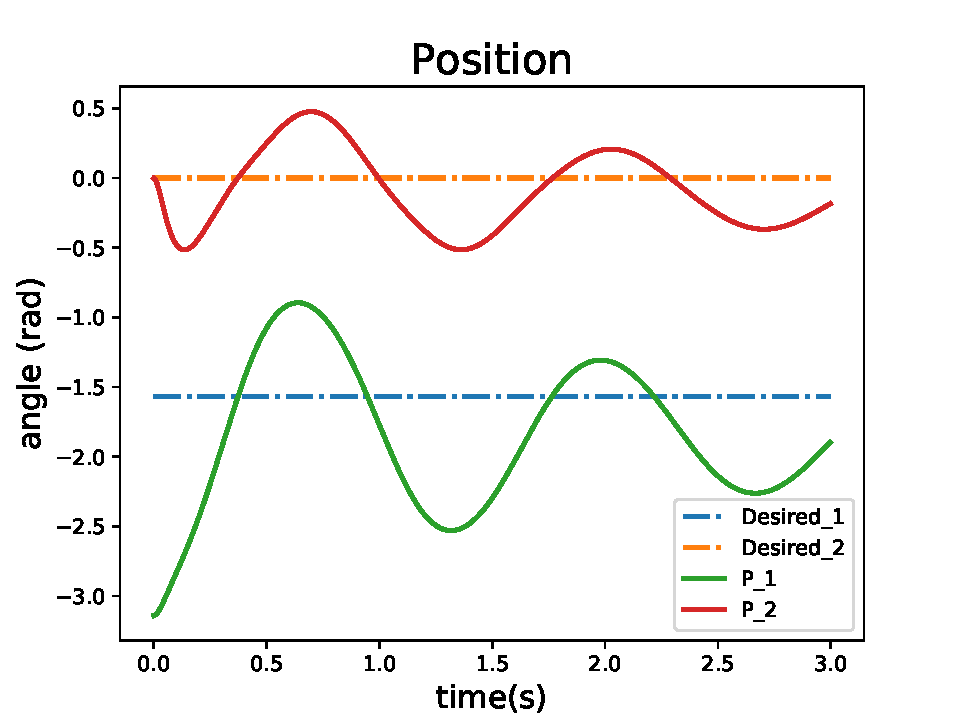
\includegraphics[width=.32\linewidth]{figures/P-Regler0.pdf}
	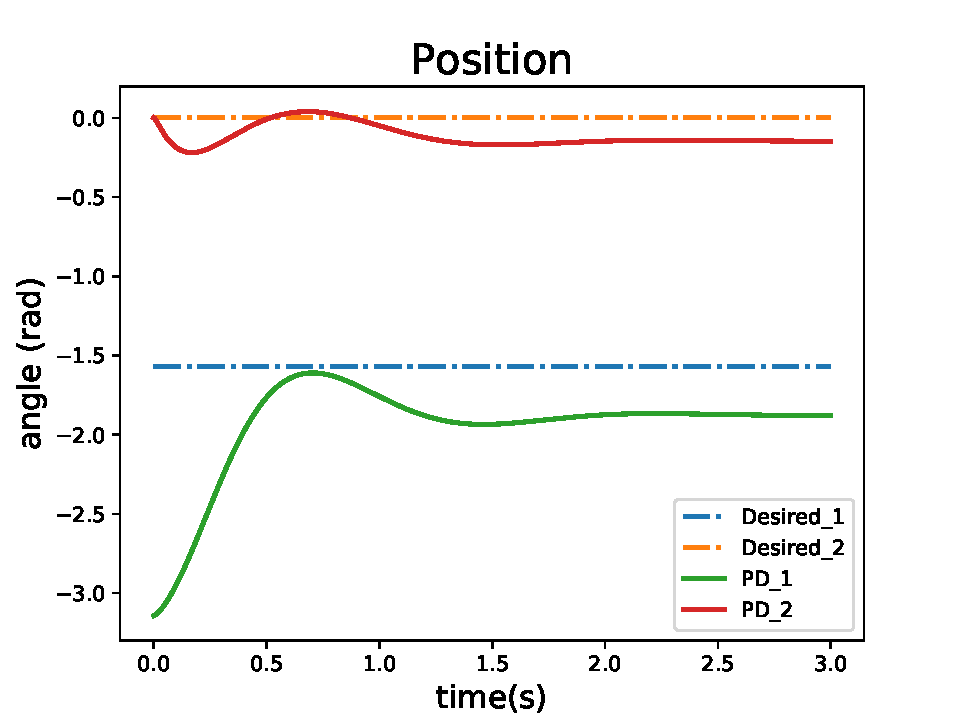
\includegraphics[width=.32\linewidth]{figures/PD-Regler0.pdf}\\
	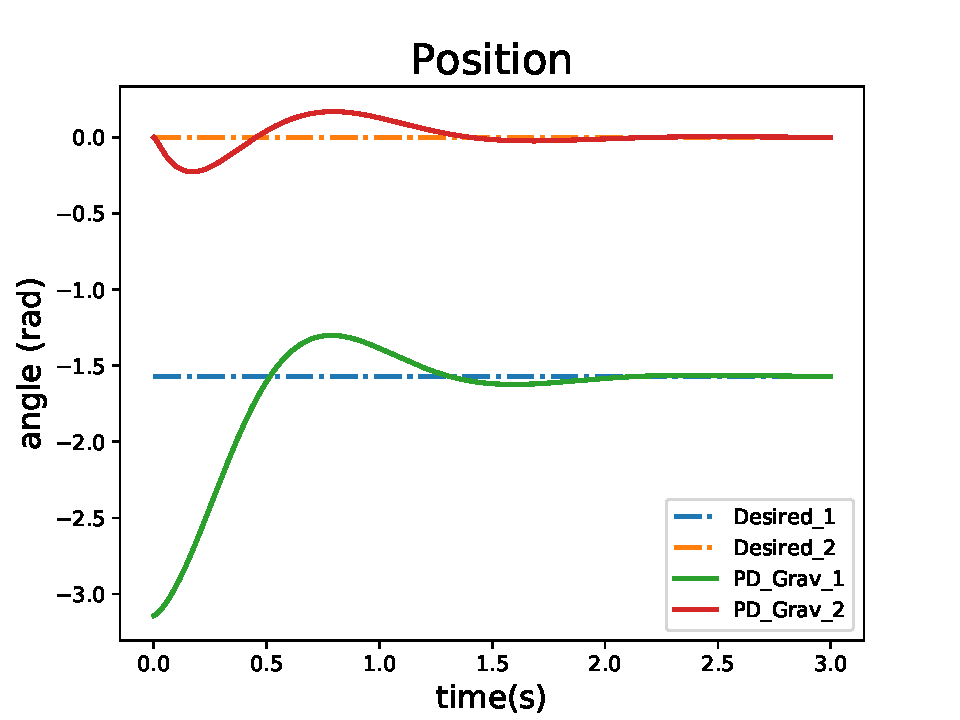
\includegraphics[width=.32\linewidth]{figures/PD-Grav-Regler0.pdf}
	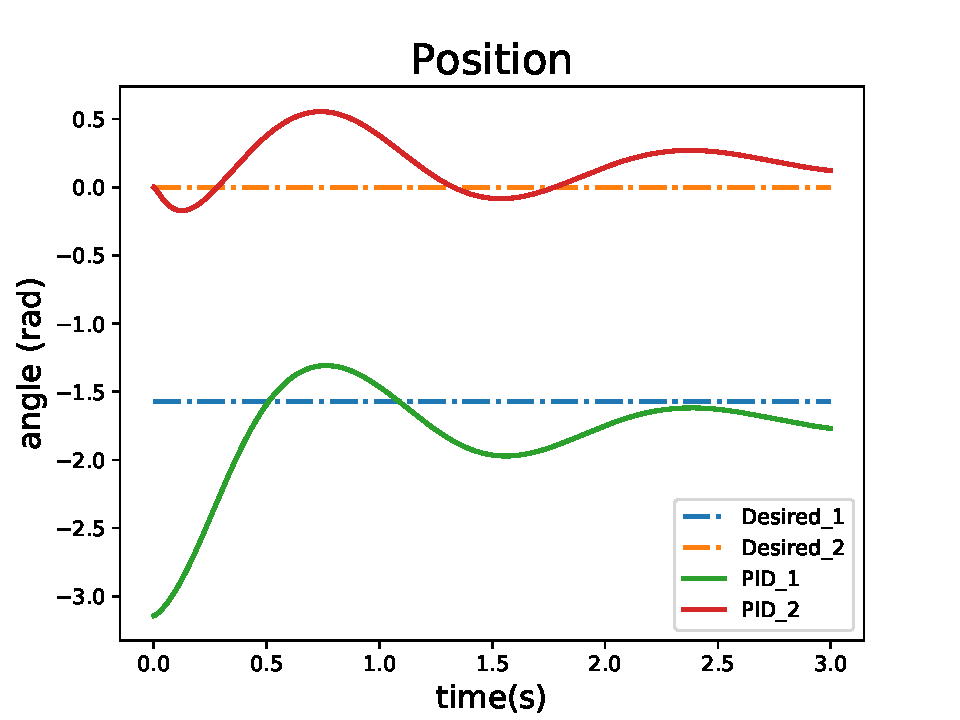
\includegraphics[width=.32\linewidth]{figures/PID-Regler0.pdf}
	%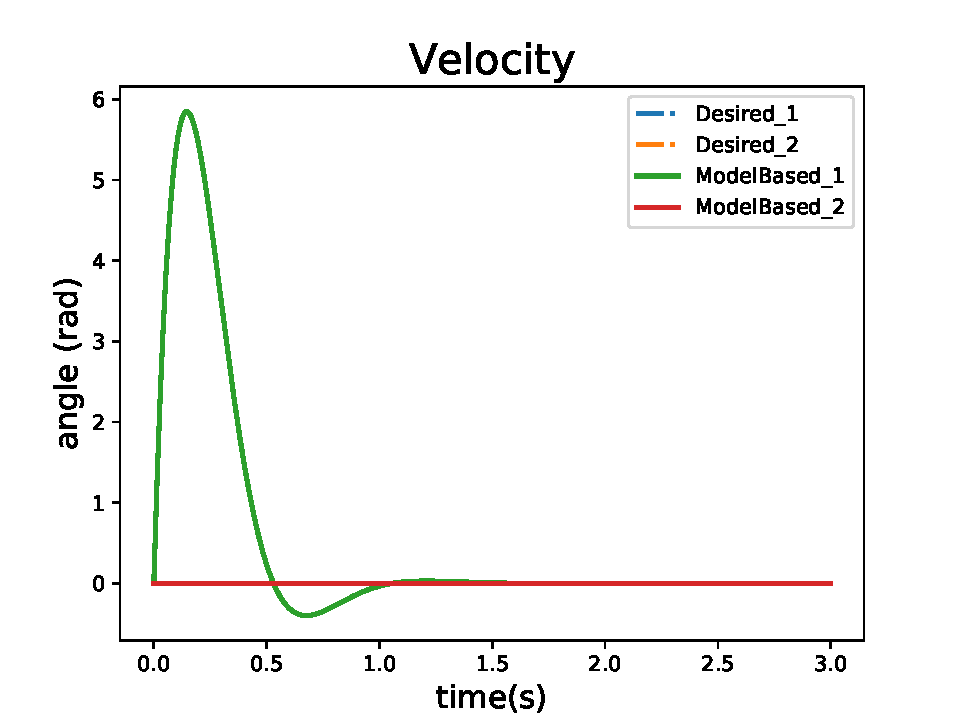
\includegraphics[width=.4\linewidth]{figures/Model-Based-Regler1.pdf}
\end{center}
	The results show that neither the P-controller nor the PID-controller reach the second desired position in the given time frame, on the other hand, it's easy to see that P controller takes a long time to get into the right position, even more it oversteers its destination by way more than the others. The PD controller gets fast to near zero velocity but stays obviously a little bit under his desired position. That's due to gravity, to compensate that the PD-Gravity controller comes with an extra term of $g(q)$. Its velocity gets as fast to zero as PD but it reaches the destination point. PID is far slower than PD but does not have such high overshoot like P-control. In PID control the difference between PD-1 and PD-2 seem bigger than within the others. But nevertheless, we would choose PID for some tasks due to its slowness, parts of the robot won't wear off this quick. Sometimes a slower robot is better than nothing, but in some situations it's essential to have a quick responsive robot. In these scenarios we would recommend to use a PD-Gravity controller, because it quickly approaches its destination and has little overshoot.
	%TODO: references
%\begin{figure}[h]
%\begin{subfigure}%{width=.5\linewidth}
%	\centering
%	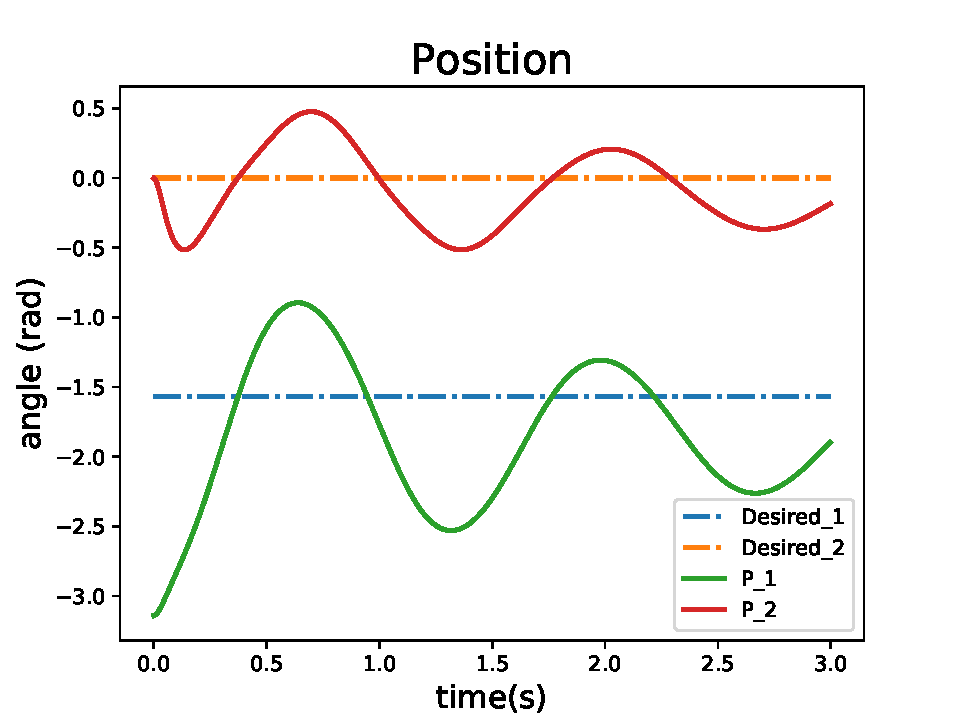
\includegraphics[width=.5\linewidth]{figures/P-Regler0.pdf}
%	\caption{Velocity Plot of a P-controller}
%	\label{P-Control}
%\end{subfigure}
%\begin{subfigure}%{width=.5\linewidth}
%	\centering
%	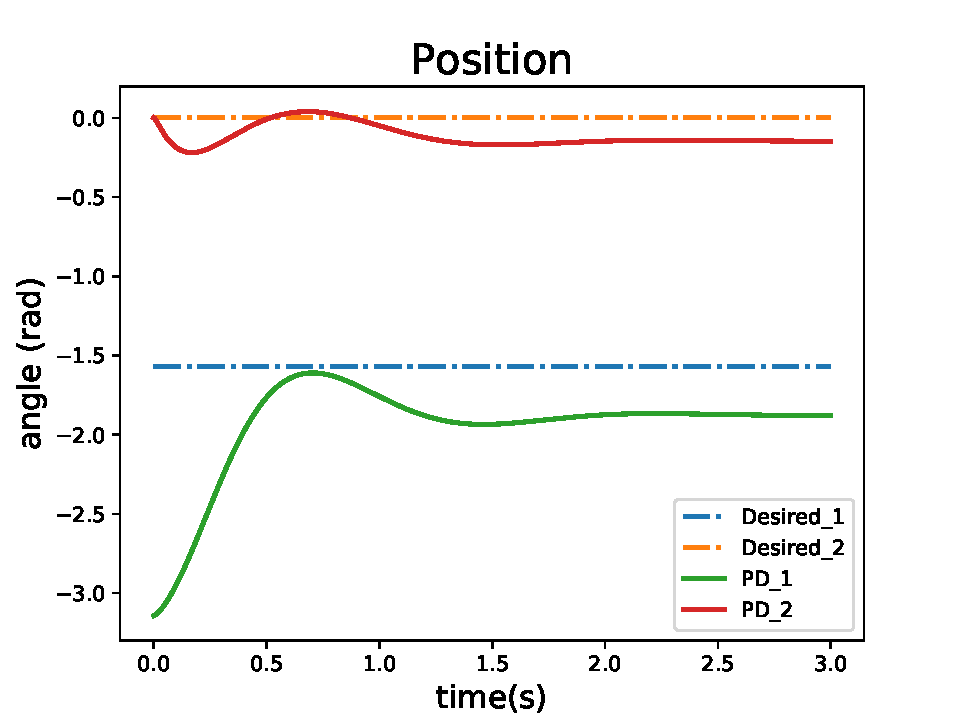
\includegraphics[width=.5\linewidth]{figures/PD-Regler0.pdf}
%	\caption{Velocity Plot of a PD-controller}
%	\label{PD-Control}
%\end{subfigure}
%	\caption{Velocitiy Plots of different controller}
%\end{figure}
\end{answer}
		
	\end{question}
	
	%----------------------------------------------
	
	\begin{question}{Tracking Trajectories}{4}
		Repeat the same experiment but this time use the provided time-varying target trajectory. Create (max 4) plots that compare the different control strategies and analyze the results. In your analysis discuss the overall performance and which controllers track the desired trajectory nicely. Additionally discuss which controller you would choose and why.
		
\begin{answer}
	\begin{center}
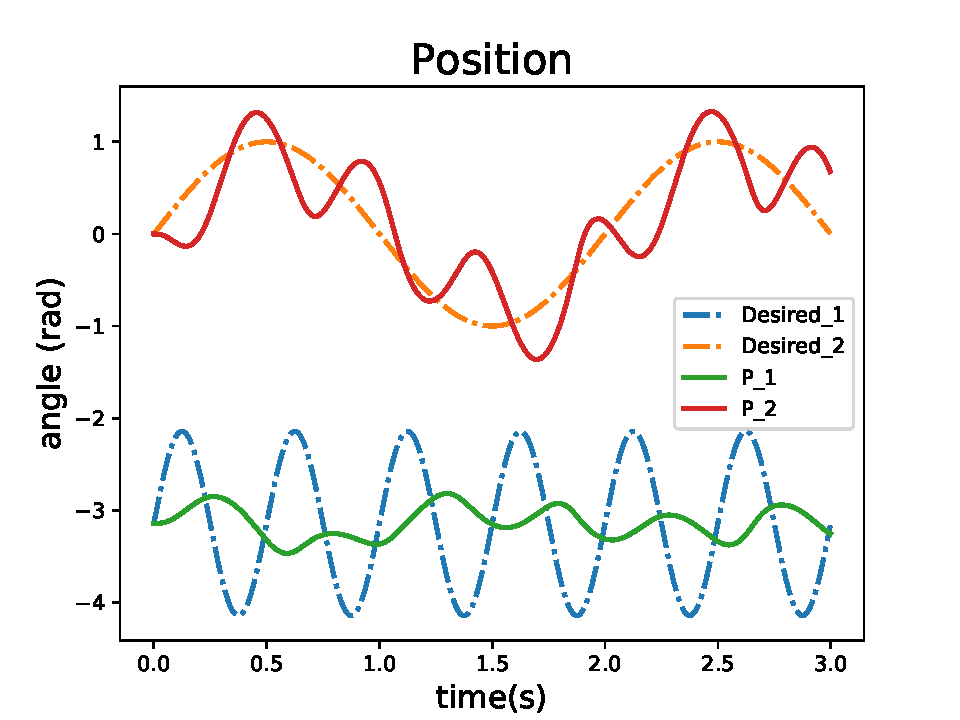
\includegraphics[width=.32\linewidth]{figures/traj/P-traj0.pdf}
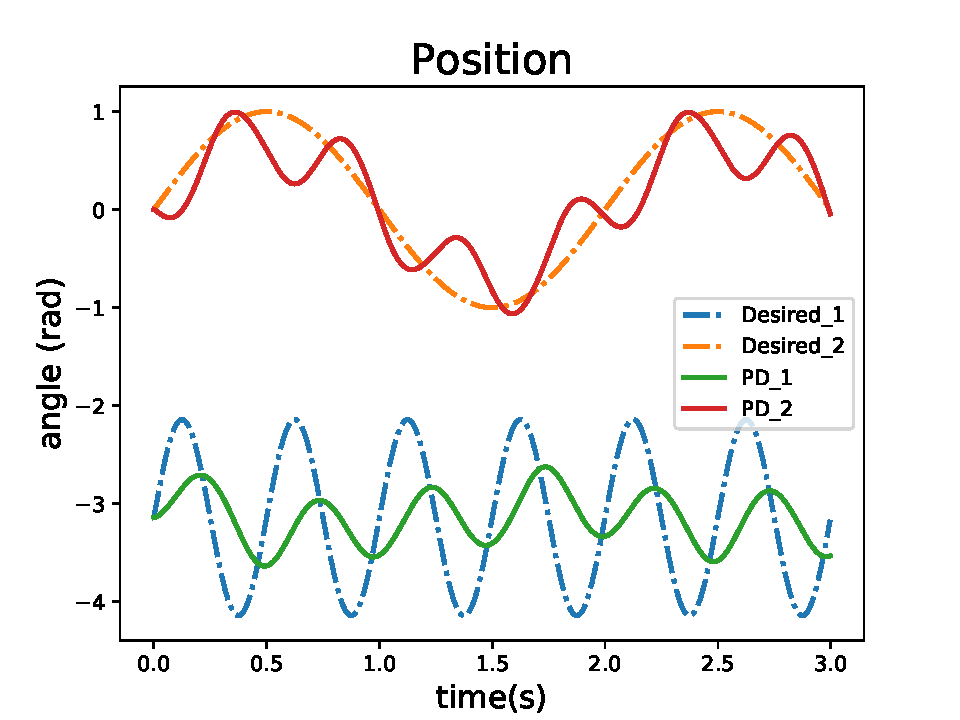
\includegraphics[width=.32\linewidth]{figures/traj/PD-traj0.pdf}\\
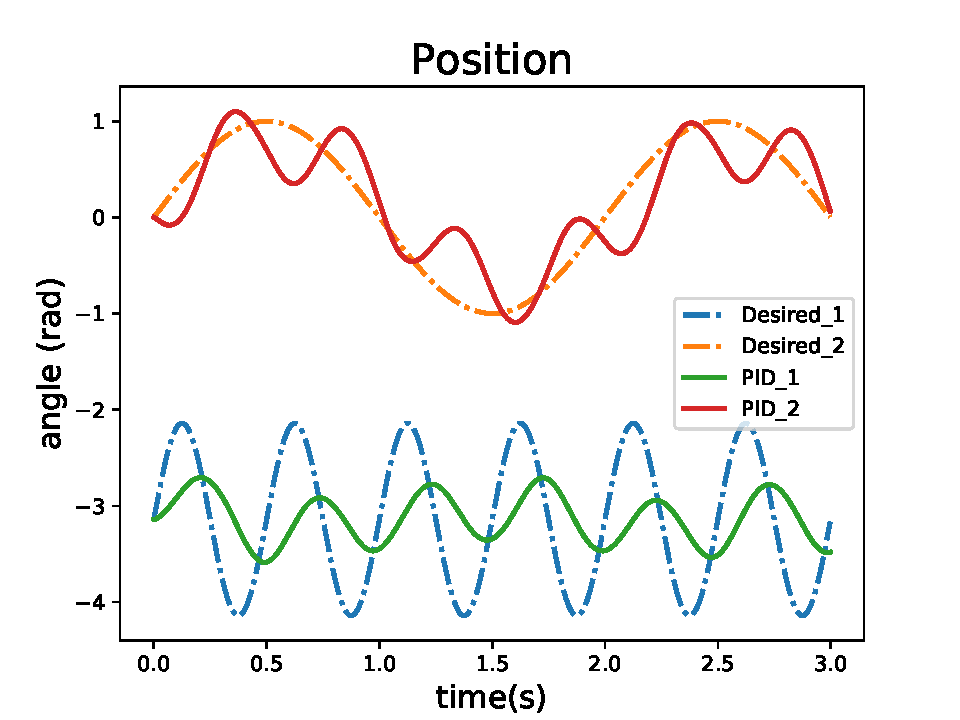
\includegraphics[width=.32\linewidth]{figures/traj/PID-traj0.pdf}
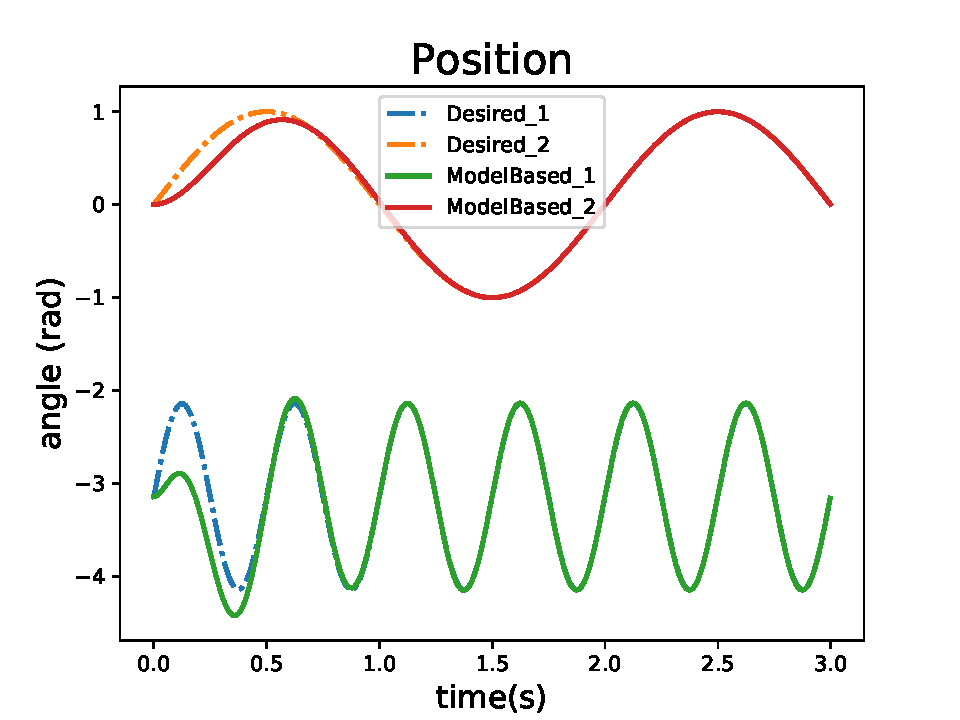
\includegraphics[width=.32\linewidth]{figures/traj/Model-Based-traj0.pdf}
	\end{center}

While tracking the trajectory, all controllers behave in a similar way. the all oscilate around the wanted curve. The difference between them is very small, so even the PD controller which performed very well in the last task can't trace the trajectory very well. This behaviour is actually pretty bad compared to a model based controller, which fits the curve nearly perfect after just a little over half a second.
\end{answer}
		
	\end{question}
	
	%----------------------------------------------
	
	\begin{question}{Tracking Trajectories --- High Gains}{4}
		Repeat the same experiment (using the provided trajectory) but this time multiply the gains by ten. Create plots that compare the different control strategies and analyze the results. In your analysis discuss the overall performance and compare it to the previous case. Are there any drawbacks of using high gains?
		
\begin{answer}
	\begin{center}
		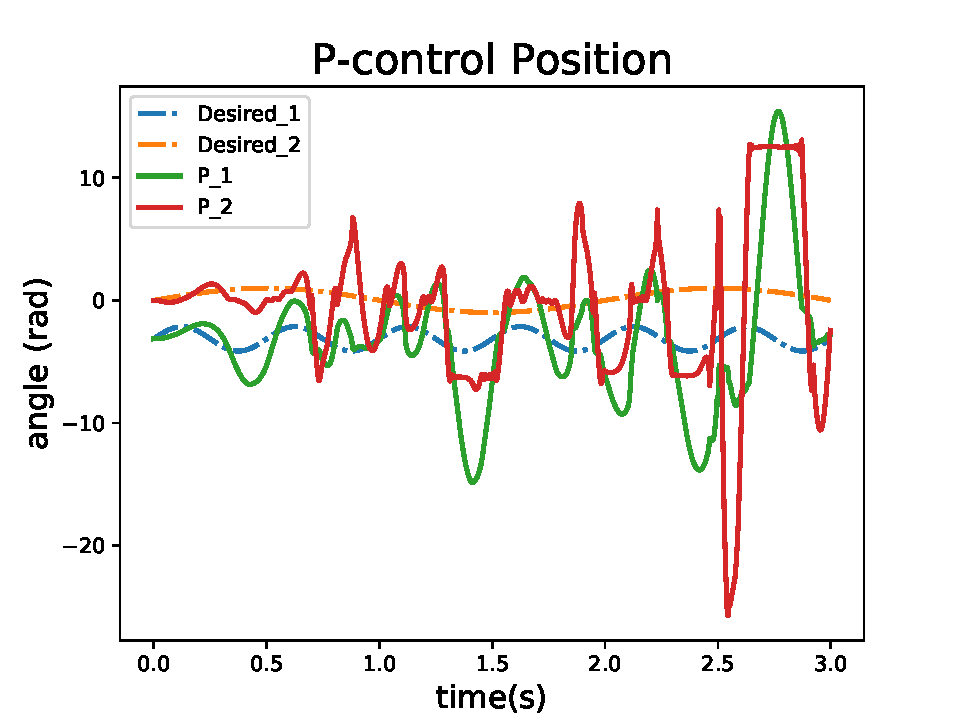
\includegraphics[width=.32\linewidth]{figures/traj/P-gain-0.pdf}
		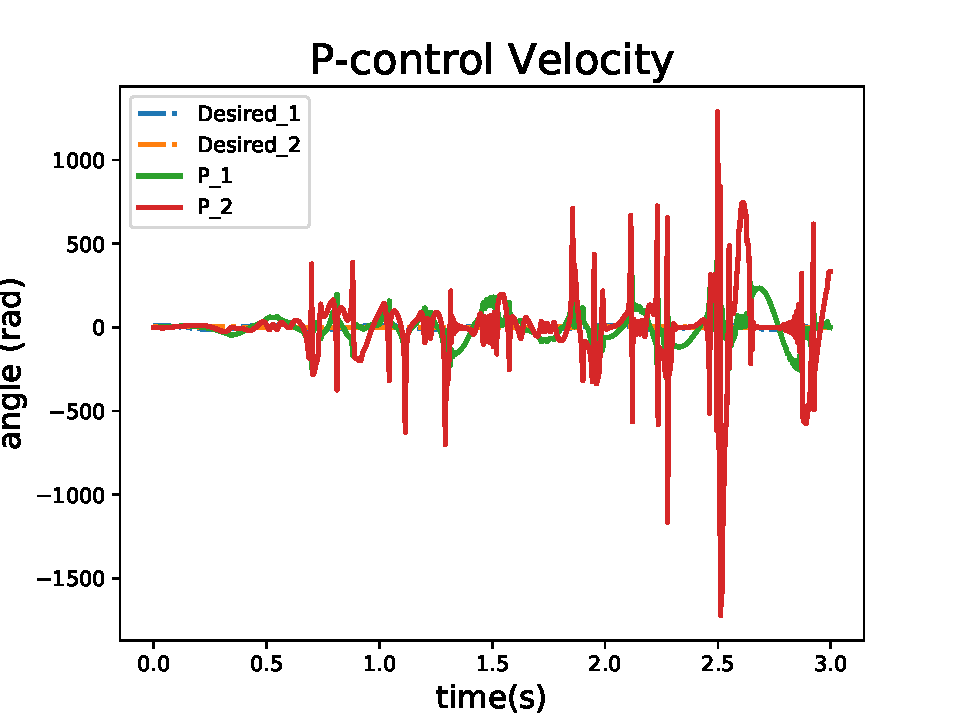
\includegraphics[width=.32\linewidth]{figures/traj/P-gain-1.pdf}\\
		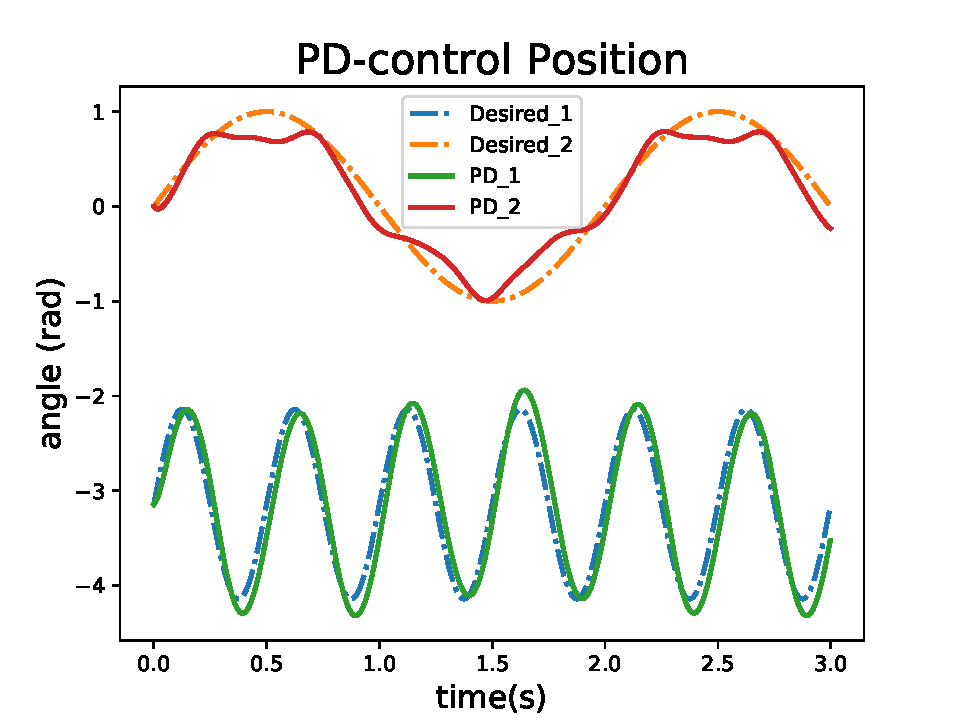
\includegraphics[width=.32\linewidth]{figures/traj/PD-gain-0.pdf}
		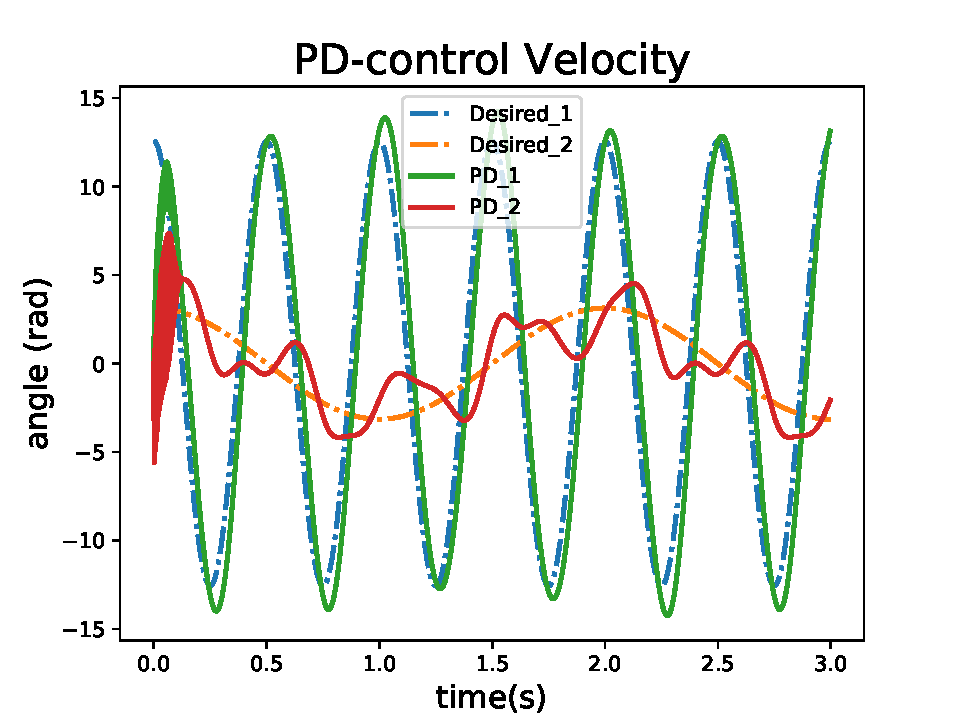
\includegraphics[width=.32\linewidth]{figures/traj/PD-gain-1.pdf}
	\end{center}
With higher gains, it's easier to overshoot the target, that's easy to see with the P-Control, while trying to get closer to the target, the difference and velocity increases. PD-, PD-Gravity- and PID control look fairly similar to each other, but have a way better approximation of the desired values than the controls without the gain. But one important note is the velocity in all of these controllers. The complete red part in the beginning of the controlled sequence is hanging rapidly. That's bad for both, analysis and real parts, that means that huge gains are costly, make the robot very stiff and dangerous.

\end{answer}
		
	\end{question}
	
	%----------------------------------------------
	
	\begin{question}[bonus]{Task Space Control}{5}
		The robot must now reach a desired position in task space $\vec{x_\textrm{end}}={[-0.35,1.5]}$. In class we derived the Jacobian transpose, Jacobian pseudo-inverse, and Jacobian pseudo-inverse with damping methods. All of them are implemented in \texttt{my\_taskSpace\_ctl.py}. You are asked to implement also the null-space task prioritization method with a null-space resting posture $\vec q=[0,\pi]$. Run the simulation and plot the initial and final configuration of the robot. Then, change the resting posture to $\vec q=[0,-\pi]$ and redo the plots. Analyze in a couple of sentences your observation. Use the same damping coefficient $10^{-6}$ and include a code snippet to your solutions.
		
\begin{answer}
%TODO
\end{answer}
		
	\end{question}
	
\end{questions}

